%%% TITLE AND AUTHORS %%%%%%%%%%%%%%%%%%%%%%%%%%%%%%%%%%%%%%%%%%%%%%%%%%%%%%%%%
\title[Final Project]{
 Final Project \\
 \small{and some examples}
}
\author[]{Szymon Talaga and Mikołaj Biesaga} % Your name
\institute[ISS UW]{
 The Robert Zajonc Institute for Social Studies \\ University of Warsaw \\
 \medskip
 \textcolor{blue}{\href{mailto:stalaga@uw.edu.pl}{stalaga@uw.edu.pl}} \\
 \textcolor{blue}{\href{mailto:m.biesaga@uw.edu.pl}{m.biesaga@uw.edu.pl}}
}
\date{\today} % Date, can be changed to a custom date

%%% SLIDES %%%%%%%%%%%%%%%%%%%%%%%%%%%%%%%%%%%%%%%%%%%%%%%%%%%%%%%%%%%%%%%%%%%%
\frame{\titlepage}

\section{Final project}

\begin{frame}{Possible forms of the project}
\begin{enumerate}
 \item \textbf{Research project proposal.}
 A short proposal for a research project using some of the methods we discussed in the class. Details are discussed
 in \textit{Structure of the proposal} section.
 \item \textbf{Simple research project and report.}
 Simple data-driven project in which you gather some data from an external web-based source (i.e. from an API or through webscraping), process it and use it to answer a simple research question. Details are discussed in
 \textit{Structure of the project} section.
\end{enumerate}
\end{frame}

\begin{frame}{Structure of the proposal | general information}
\begin{itemize}
 \item \textbf{Introduction and problem statement.}
 This section should explain what is the project about in general and why the given problem matters. The significance of the problem may be justified both in terms of its theoretical/scientific or societal/business relevance.
 \item \textbf{Research question.}
 What is the specific research question you will try to answer in the project? It can be either formulated as a strict hypothesis or as an exploratory question (i.e. not assuming any particular effect or mechanism).
 \item \textbf{Research methods.}
 This section should discuss, at a general level, what data do you plan to use and how will analyze it. In particular, you should clearly explain why the data and methods you chose will allow you to answer your research question.
\end{itemize}
\end{frame}

\begin{frame}{Structure of the proposal | research methods}
\begin{itemize}
 \item \textbf{Data collection.} What is the data you are planning to use?
 Where is it stored and how do you plan to obtain/extract it?
 Are there any possible obstacles and if there are what can be done to minimize the risk of failure?
 \item \textbf{Data preprocessing and storage.}
 How will you preprocess data and in what format will store it for later use? For instance, when scraping you may decide to data gathered from
 every individual website to a JSON object and store all data in
 \texttt{.jl} file (JSON lines).
 \item \textbf{Analytic methods.}
 What analytic methods will you apply to your data in order to answer your question? This may include some methods that we discussed in the class
 (i.e. sentiment analysis or some other natural language processing methods),
 but you should also use your general statistical knowledge to decide how you want to model your final data.
\end{itemize}
\end{frame}

\begin{frame}{Structure of the project}
\begin{itemize}
 \item The project should consist of two main items:
 \begin{enumerate}
 \item \textbf{Notebook} with code and description of the project.
 More on that below.
 \item File with the \textbf{raw data} as was extracted from the external data source (e.g. API or webpage).
 \end{enumerate}
 \item The notebook should include a short introduction describing the problem and why it is significant.
 \item The specific research question should be introduced.
 \item Data source should be discussed. In particular in relation to the research question.
 \item Data analysis methods should be discussed, also in relation to the research question.
 \item Code and text should be mixed in the notebook in a way that facilitates understanding of the adopted research methods and obtained results.
\end{itemize}
\end{frame}

\begin{frame}{Things to remember}
\begin{itemize}
 \item Make sure you will be able to gather data legally.
 For instance, if you want to scrape some websites you should try to determine whether they allow scraping. You can check this by
 looking at the so-called \texttt{robots.txt} of a website.
 It can be found at \texttt{<url>/robots.txt}. For instance,
 you can see Facebook configuration at \texttt{facebook.com/robots.txt}.
 \item Be kind for your data source. If there is a platform that exposes an API you should use it instead of scraping data directly from its webpage.
 \item Think about proper format for storing data. If you plan to use your data to compute a statistical model in SPSS may be JSON lines are not the best and you should consider storing your data as a simple CSV file?
\end{itemize}
\end{frame}

\begin{frame}
    \frametitle{Formal requirements}
    \begin{itemize}
        \item Regardless whether you chose a project or a proposal the deadline for submitting it is on \textbf{7.02.2020 23:59:59}.
        \item If you decide to submit a project please send us two files: the notebook and the raw data file. Please, remember to rename them properly FP\_<SURNAME>\_<NAME>.ipynb and FP\_<SURNAME>\_<NAME>.jl (the data file might have the format of your choice, it doesn't have to be a JSON line file).
        \item If you decide to submit a proposal your work should not be shorter than 3 pages and not longer than 5 (interline: single, font size: 12). Please, remember to rename your file properly FP\_<SURNAME>\_<NAME>.docx.
    \end{itemize}
\end{frame}

\section{SMART}


\subsection{Data gathering}
\begin{frame}
 \only<1>{
 \frametitle{Data gathering}
 \begin{itemize}
 \item Sources Selection
 \item Facebook Data Collection
 \item Webscraping
 \end{itemize}
 }
 \only<2>{
 \frametitle{Soruces Selection}
 \begin{table}
 \resizebox{\framewidth}{!}{
 \begin{tabular}{|l|l|c|c|}
 \hline
 Source Name & Origin & Facebook Likes & Facebook Followers \\ 
 \hline
 The Parliament Magazine & UE & $4,502$ & $4,848$ \\
 EUobserver & UE & $141,859$ & $142,034$ \\
 Euronews English & UE & $2,040,663$ & $2,083,956$ \\
 EURACTIV & UE & $40,179$ & $42,370$ \\
 POLITICO Europe & UE & $143,028$ & $149,377$ \\
 Russia Today & Russia & $5,510,636$ & $5,600,911$ \\
 Sputnik News & Russia & $1,252,461$ & $1,269,249$ \\
 Daily Mirror & UK & $3,114,909$ & $3,073,220$ \\
 The Guardian & UK & $8,160,962$ & $8,072,817$ \\
 Daily Express & UK & $1,334,230$ & $1,349,291$ \\ 
 \hline
 \end{tabular}
 }
 \end{table}
 }
 \only<3>{
 \frametitle{Facebook Data Collection}
 
\includegraphics[width=\framewidth]{png/sotrender.png}
 }
\end{frame}
\begin{frame}[fragile]
 \frametitle{Facebook Data Collection}
 \tiny
 \begin{minted}{json}
{
 "fb_post_id":"326683984410_10155067229969411",
 "type":"link",
 "author":"page",
 "date":"2017-01-01",
 "hour":"03:00:00",
 "text":"World markets are finishing unexpectedly well in a year full of political
 shocks",
 "reactions_like":0,
 "reactions_angry":0,
 "reactions_haha":0,
 "reactions_wow":0,
 "reactions_sad":0,
 "reactions_love":0,
 "shares":18,
 "is_respond":0,
 "votes":0,
 "ini":455,
 "likes":127,
 "comments":10,
 "response_time":0,
 "was_deleted":0,
 "name":"RT",
 "created_at":"2017-01-01 03:00:00",
 "link_title":"Oil, equities, emerging markets end turbulent year on high note",
 "link_content":"rt.com",
 "link":"https://www.rt.com/business/372285-oil-equities-emerging-markets-results/",
 "url":"https://facebook.com/326683984410_10155067229969411"
}
 \end{minted}
\end{frame}
\begin{frame}
 \only<1>{
 \frametitle{Webscraping}
 
\includegraphics[width=\framewidth]{png/scrapy.png}
 }
\end{frame}
\begin{frame}[fragile]
 \frametitle{Webscraping}
 \tiny
 \begin{minted}{json}
{
"content": "\u201cThe US will consider sanctions off-ramps for any Venezuelan senior 
military officer that stands for democracy and recognizes the constitutional government 
of President Juan Guaido,\u201d Bolton said in a tweet. \u201cIf not, the international 
financial circle will be closed off completely. Make the right choice!\u201d\n\nEarlier,
Bolton said that the United States has no plans for an imminent military intervention
in Venezuela, but all options with regard to the situation in the Latin American country
remain on the table.\n\nREAD MORE:\n\nPompeo Demands That Venezuela's Military Stop
Blocking US Aid\n\nJuan Guaido proclaimed himself Venezuela's interim president
in January. The US, Canada, and several other countries immediately recognised him.
Nicolas Maduro has meanwhile called him a US \"puppet\" and accused Washington of
organising a coup in Venezuela.",
"figcaptions": ["US National Security Adviser John Bolton"],
"lead": "The US government is offering to end sanctions on senior Venezuela Army officers
who switch their allegiance to National Assembly Speaker Juan Guaido, whom Washington
recognizes as president, National Security Adviser John Bolton said on Wednesday.",
"published_at": "2019-02-06T23:38:00", 
"tags": ["latin america"], 
"title": "Washington Offers To Lift Sanctions on Venezuela Officers Shifting to Guaido", 
"updated_at": "2019-02-06T23:43:00", 
"source_name": "Sputnik", 
"timestamp": "2019-02-06T21:30:00", 
"fb_post_id": "357990416180_10156861691866181", 
"url": "https://sputniknews.com/latam/201902061072192247-us-venezuela-bolton-sanctions/",
"final_url": "https://sputniknews.com/latam/201902061072192247-us-venezuela-bolton-
sanctions/",
"content_id": "48eb898bdc0e10912cfc5947325103e5",
"content_length": 844, 
"scraped_at": "2019-06-04T10:21:03.715388", 
"lang": "en", 
"polarity": {"neg":0.083,"neu":0.903,"pos":0.014,"compound":-0.8398}
}
 \end{minted}
\end{frame}
\begin{frame}
 \only<1>{
 \frametitle{Data Storage}
 
\includegraphics[width=\framewidth]{png/mongodb.png}
 }
 \only<2>{
 \frametitle{Webscraping}
 \begin{table}
 \resizebox{\framewidth}{!}{
 \begin{tabular}{|l|l|c|c|c|}
 \hline
 Source Name & Origin & Facebook Likes & Facebook Followers & Articles \\ 
 \hline
 The Parliament Magazine & UE & $4,502$ & $4,848$ & $887$\\
 EUobserver & UE & $141,859$ & $142,034$ & $2,663$ \\
 Euronews English & UE & $2,040,663$ & $2,083,956$ & $19,224$ \\
 EURACTIV & UE & $40,179$ & $42,370$ & $4,472$ \\
 POLITICO Europe & UE & $143,028$ & $149,377$ & $4,212$ \\
 Russia Today & Russia & $5,510,636$ & $5,600,911$ & $28,987$ \\
 Sputnik News & Russia & $1,252,461$ & $1,269,249$ & $42,927$ \\
 Daily Mirror & UK & $3,114,909$ & $3,073,220$ & $41,553$ \\
 The Guardian & UK & $8,160,962$ & $8,072,817$ & $35,875$ \\
 Daily Express & UK & $1,334,230$ & $1,349,291$ & $21,898$ \\ 
 \hline
 \end{tabular}
 }
 \end{table}
 }
\end{frame}
\subsection{Topic discovery}
\begin{frame}
 \only<1>{
 \frametitle{Topic discovery}
 \begin{itemize}
 \item Latent Dirichlet Allocation
 \item Filltering topics
 \end{itemize}
 }
 \only<2>{
 \frametitle{Latent Dirichlet Allocation}
 
\includegraphics[width=\framewidth]{png/gensim.jpeg}
 }
 \only<3>{
 \frametitle{Latent Dirichelt Allocation}
 \begin{table}
 \resizebox{\framewidth}{!}{
 \begin{tabular}{|p{10cm}|l|c|}
 \hline
 Title & Source & p \\ 
 \hline
 Golden Globes 2018: The full list of winners by category & Euronews English & $.92$ \\
 \hline
 Donald Glover to star in Disney’s Lion King remake - and James Earl Jones returns as Mufasa & Daily Mirror & $.91$ \\
 \hline
 Star Wars’ saga turns 40 & Euronews English & $.89$ \\
 \hline
 Flower of the Universe: hear Sade’s first new music in eight years & The Guardian & $.87$ \\
 \hline
 Final Beauty and the Beast trailer featuring John Legend and Ariana Grande’s duet is most magical of them all & Daily Mirror & $.86$ \\
 \hline
 Music Legends Unite in Tributes to 'Father of Rock and Roll' Chuck Berry & Sputnik & $.85$ \\
 \hline
 K-pop group BTS top US album charts & Euronews English & $.85$ \\
 \hline
 'Beren and Lúthien': JRR Tolkien book released a century after he wrote it & Russia Today & $.84$ \\
 \hline
 Emma Stone wins best actress Oscar for La La Land & The Guardian & $.82$ \\
 \hline
 Joaquin Phoenix spotted in traditional clown costume on set of Joker movie & Daily Mirror & $.83$ \\
 \hline
 \end{tabular}
 }
 \end{table}
 }
 \only<4>{
 \frametitle{Wordclouds}
 \begin{center}
 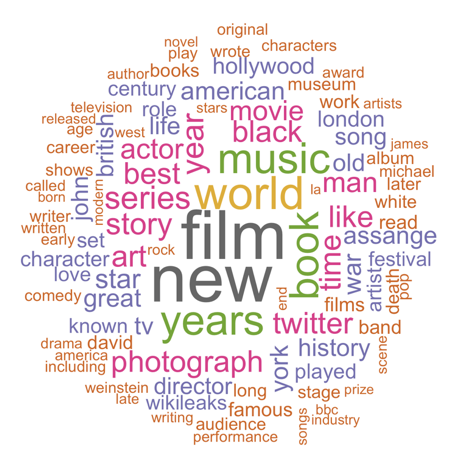
\includegraphics[height=8cm]{png/wordcloud_entertainment.png}
 \end{center}
 }
\end{frame}
\subsection{Sentiment Analysis}
\begin{frame}
 \only<1>{
 \frametitle{Sentiment Analysis}
 \begin{itemize}
 \item VADER - lexicon and rule based sentiment Analysis
 \item Within-topic sentiment relative variance
 \item SoTrender Social Media Inteactivity
 \end{itemize}
 }
 \only<2>{
 \frametitle{VADER - lexicon and rule based sentiment}
 $sentiment = compound \times (1-neutral)$
 }
 \only<3>{
 \frametitle{Relative variance}
 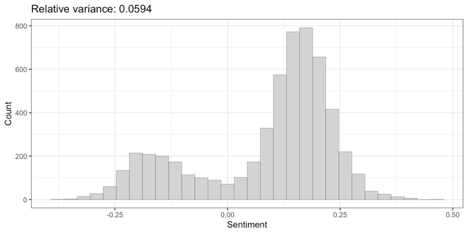
\includegraphics[height=4cm]{png/relative_variance_entertainment.png}
 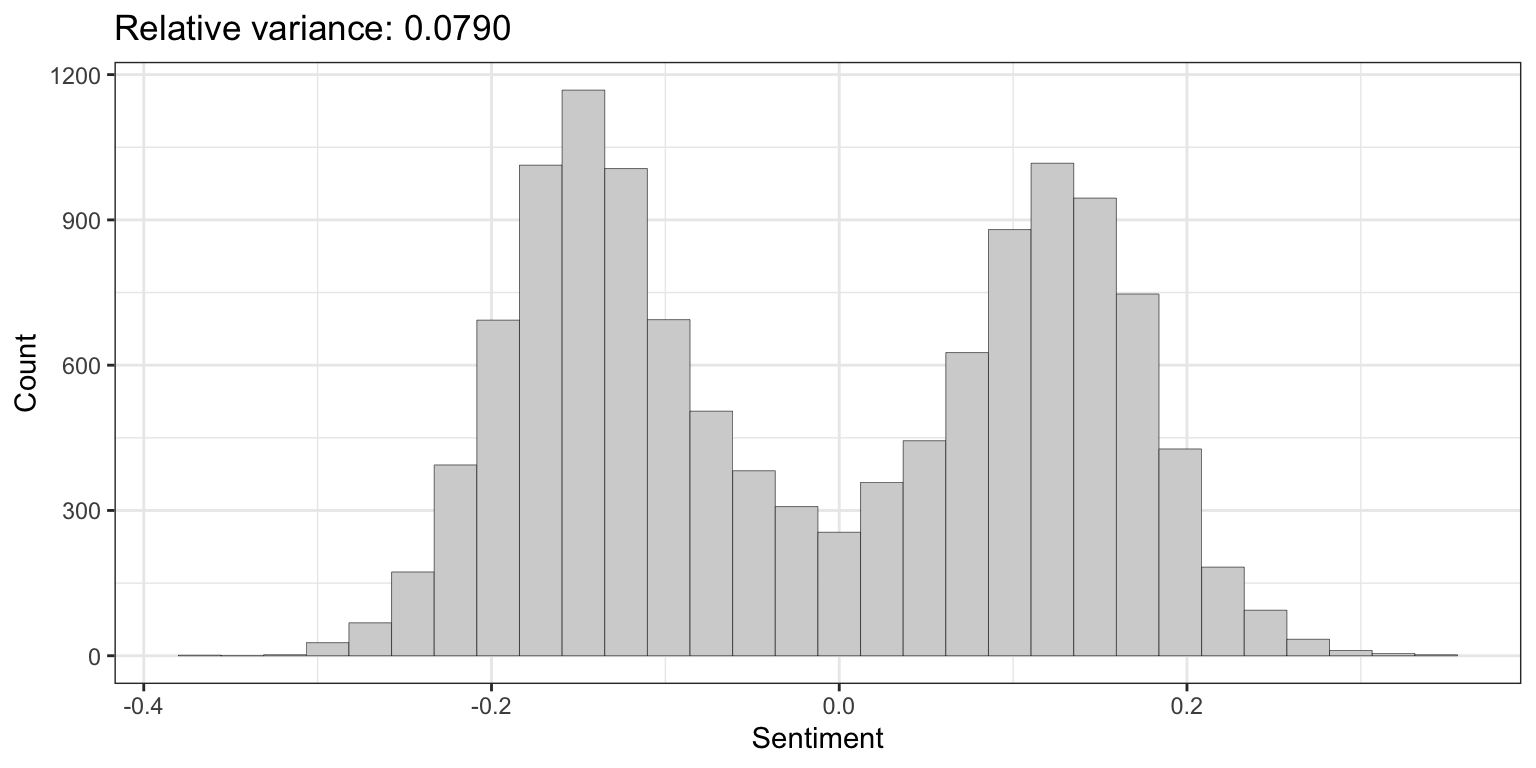
\includegraphics[height=4cm]{png/relative_variance_trump.png}
 }
 \only<4>{
 \frametitle{SoTrender Social Media Interactivty Index}
 \begin{enumerate}
 \item[]$INI = ln(1+n_{Likes}+4\times n_{Shares} + 16 \times n_{Comments})$
 \item[]$INI = ln(\frac{1+n_{Likes}+4\times n_{Shares} + 16 \times n_{Comments}}{\bar{x}_{INI}})$
 \end{enumerate}
 }
 \only<5>{
 \frametitle{Inteactivity and Sentiment}
 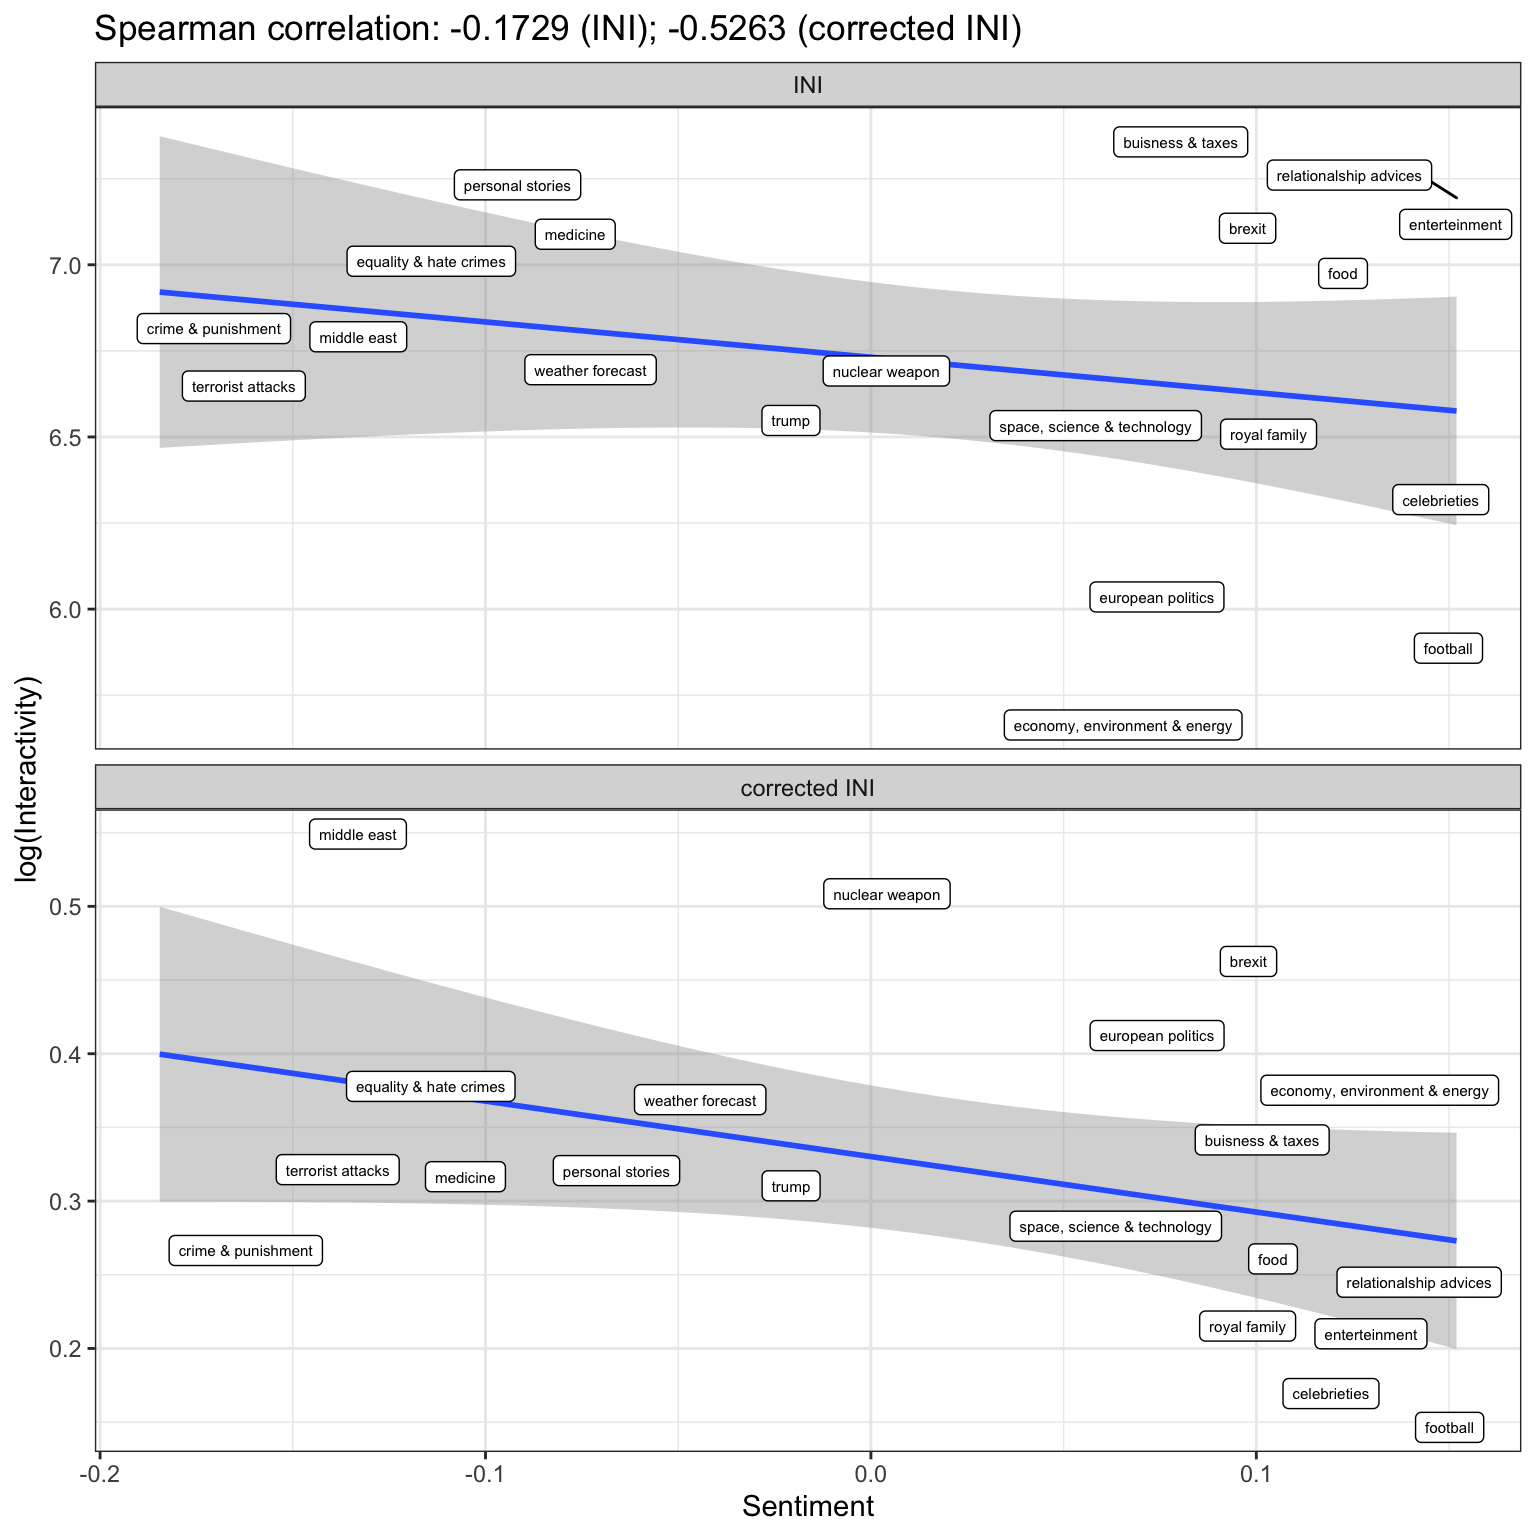
\includegraphics[height=8cm]{png/overall_analysis_sentiment_ini_trend-1.png}
 }
 \only<6>{
 \frametitle{Interactivity and Relative Varience}
 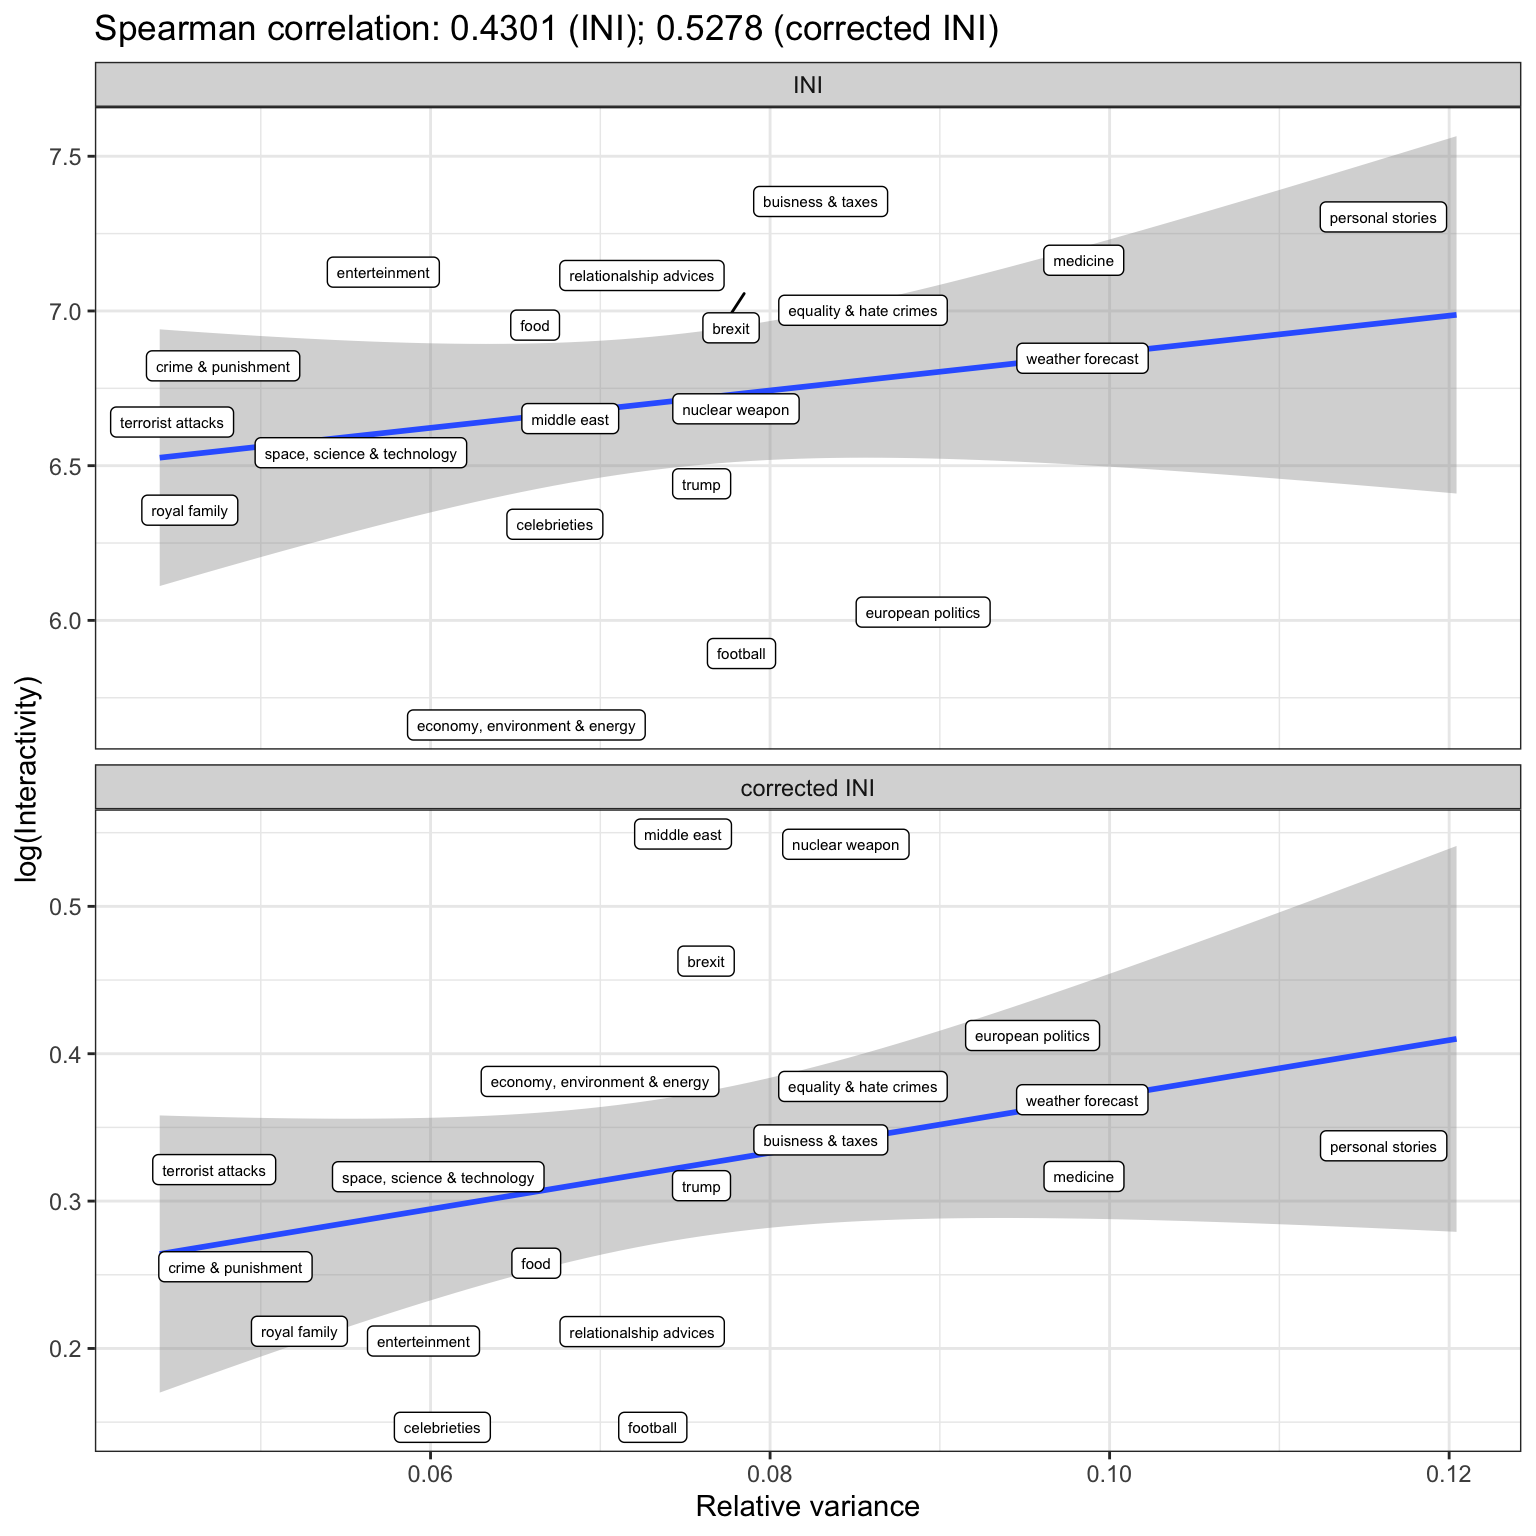
\includegraphics[height=8cm]{png/overall_analysis_ini_relative_variance_trend-1.png}
 }
\end{frame}


%%% LITERATURE %%%%%%%%%%%%%%%%%%%%%%%%%%%%%%%%%%%%%%%%%%%%%%%%%%%%%%%%%%%%%%%%
%\begin{frame}[allowframebreaks]
%\frametitle{Literature}
%\nocite{*}
%\AtNextBibliography{\footnotesize}
%\printbibliography[title=Literature]
%\end{frame}

